\chapter{Performance experiments}

The performance experiments were designed to explore the parallel performance of ABC SMC inference framework that was used in our parameter estimation and model selection tasks. Generally, ABC SMC is a time-consuming and computation-intensive task and ideally executed on large clusters. The scheduling strategy, implementation details, randomness in the algorithm and many other factors can affect the parallel efficiency. Thus, we designed a scaling-up experiment and studied a case where abnormal performance was observed.

% [MORE meanings of the performance study]

\section{Scaling-up}

First experiments are designed to illustrate the scaling-up performance. The program used here is an implementation of ABC SMC on model 5. The details of the ABC SMC settings are listed below

\begin{itemize}
    \item Prior distribution: default to log-uniform distribution [$1\times 10^{-6}$, 50] for all the 12 parameters
    \item threshold schedule: median epsilon
    \item No factors, no adaptive distance or adaptive population applied
    \item Population size is 2000, with 20 generations
\end{itemize}

% [HOW PYABC parallelise the sampling]

For HPC systems like Cirrus, \verb|pyabc| uses \verb|multiprocessing| for multi-core parallel sampling. By default, if the number of cores is not specified, it will automatically read the number of available cores and use them all. Cirrus has a 36-core CPU which support hyperthreading, such that the maximal number of cores available to \verb|multiprocessing| is 72.

The experiment was executed on Cirrus, using 8, 16, 24, 36, 54 and 72 cores respectively. Each run was repeated ten times and the average execution time, required sampling numbers are recorded. Hyperthreading was enabled when using 54 and 72 cores. The access to the node that contains computation cores is exclusive, such that the execution would not be affected by other programs of operations.

The implementation of ABC SMC in \verb|pyabc| enables the parallelisation of sampling, which is the most time-consuming part. The rest part of the program is mostly not parallelised, e.g. database I/O and reductions operations. The sampling process involves sampling, perturbation and test of the acceptance criteria, which are computation-intensive.

In practice, using ABC SMC to estimate the parameters of a given model could cost up to several hundred of hours if the computational resources are limited \cite{ref:compare}. The performance experiment result could provide a reference that illustrates how the efficiency changes when scaling-up or the trade-offs in computational resources' cost and their benefit.

\subsubsection{Results}

% [scaling-up performance: speed-up and efficiency]

% [large variation in required sampling numbers]

% [possible reasons]

\begin{figure}[h]
    \begin{center}
        \resizebox{1.0\hsize}{!}{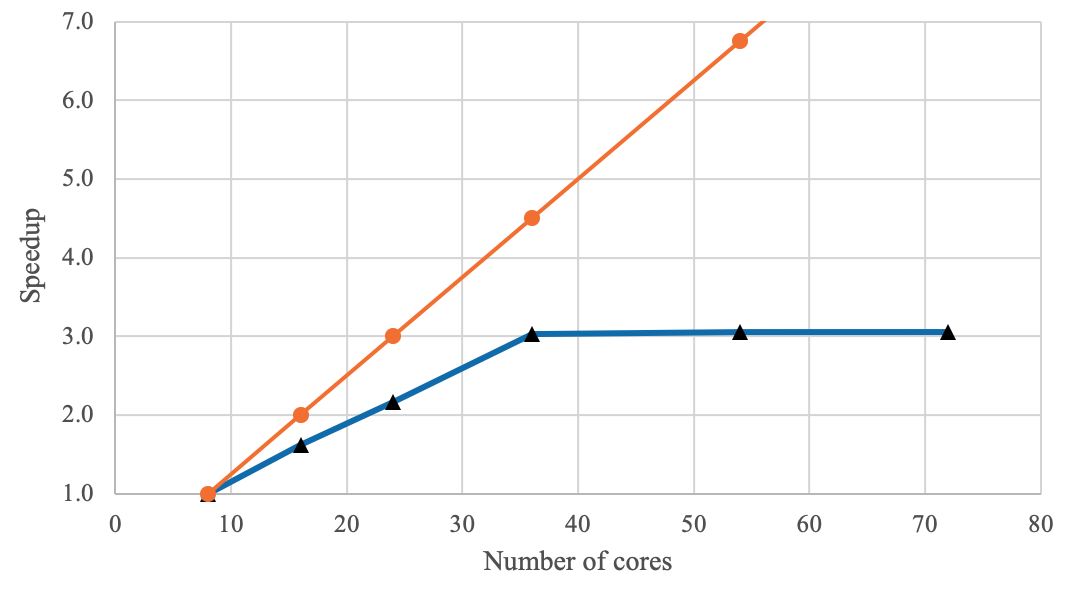
\includegraphics{fig/speedup.png}}
    \end{center}

    \caption[Speedup of the program]{Speedup of the program}
    \label{fig:speedup}
\end{figure}

The recorded execution time under different numbers of cores was used to calculate the speedup of the program (Figure \ref{fig:speedup}). Here 8-core run is regarded as the baseline for speedup and efficiency, as the serial version (using only one core) can take quite a long time to finish 10 repeats. When increasing number of cores, the execution time drops fast at first, but the decreasing trend became slower for large numbers of cores; 36, 54 and 72 cores gives nearly the same average execution time and consequently gains very close speedup values (Table \ref{table:performance}).

\begin{table}[H]
    \centering
    \begin{tabular}{|c c c c c|}
        \hline
        Number of cores & Time (second) & Avg. required samples & Speedup & Efficiency \\ [0.5ex]
        \hline\hline
        8               & 6617          & 445406.8              & 1       & 1          \\
        16              & 3926          & 590221.0              & 1.61    & 0.807      \\
        24              & 2921          & 573339.8              & 2.17    & 0.723      \\
        36              & 2096          & 446948.7              & 3.02    & 0.672      \\
        54              & 2076          & 640404.9              & 3.05    & 0.452      \\
        72              & 2071          & 768096.0              & 3.06    & 0.340      \\
        \hline
    \end{tabular}
    \caption{Performance data}
    \label{table:performance}
\end{table}

Denote the number of cores used in the ABC SMC runs as variable $p$. The speedup curve shows a linear trend when $p\leq 36$; when $p\geq 36$ the speedup stays nearly unchanged. $p=36$ is an inflexion point, where 36 is the maximum numbers available physical cores in a compute node of Cirrus. A constant drop of efficiency is observed when increasing $p$; smaller $p$ ($p<36$) gives an efficiency higher than 65\% but greater $p$ e.g. $p=72$ results in a low efficiency (34\%).

\begin{figure}[h]
    \begin{center}
        \resizebox{1.0\hsize}{!}{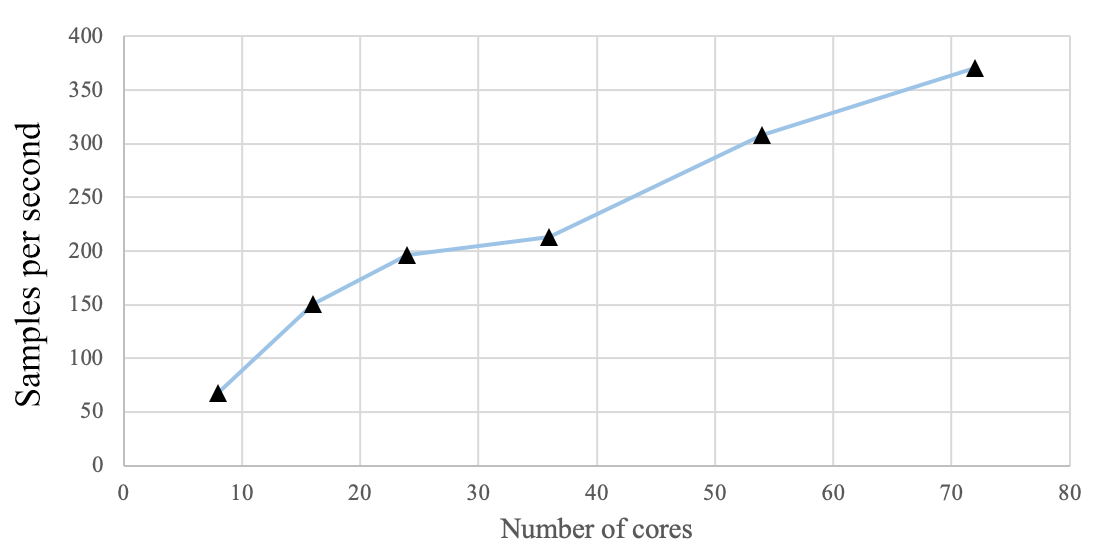
\includegraphics{fig/sample_per_time.png}}
    \end{center}

    \caption[Average samples in a second, under different number of cores]{Average samples in one second, under different number of cores}
    \label{fig:sample_per_sec}
\end{figure}

\section{Discussions}

A high variance of total required samples was observed in the scaling-up experiments: some single runs required much more samples to finish 20 populations, where they were supposed to have relatively similar average required samples such that we can compare the performance directly via speedup or efficiency.

Due to the variant required samples, our interests switched to the per-second performance, where the average sampling numbers per second under different of numbers of cores ($p$) are plotted (Figure \ref{fig:sample_per_sec}). The plot shows that even theoretical speedup stops growing when $p>36$, the average sampling numbers per second performance still get improved when using more than 36 cores. It proves that the implementation used here scales reasonably well without encountering bottleneck when using multi-core parallelisation inside one physical node.

The variant total required samples for different runs under the same setting was most likely the result of different threshold evolve path. Median epsilon schedule and randomness in the sampling process resulted in different sequences of thresholds for different runs, which means different repeated runs may have different convergency path \cite{threshold}. For example, Some runs temporarily converge to a local optimum, while the target epsilon in the next generation cannot possibly be reached if the new particles are still concentrated in the local optimum. In this case, a huge amount of sample will be drawn to find enough accepted particles, and the new generation will be able to jump out of the local optimum and have different concentrations. 

\begin{figure}[ht]
    \begin{center}
        \resizebox{1.0\hsize}{!}{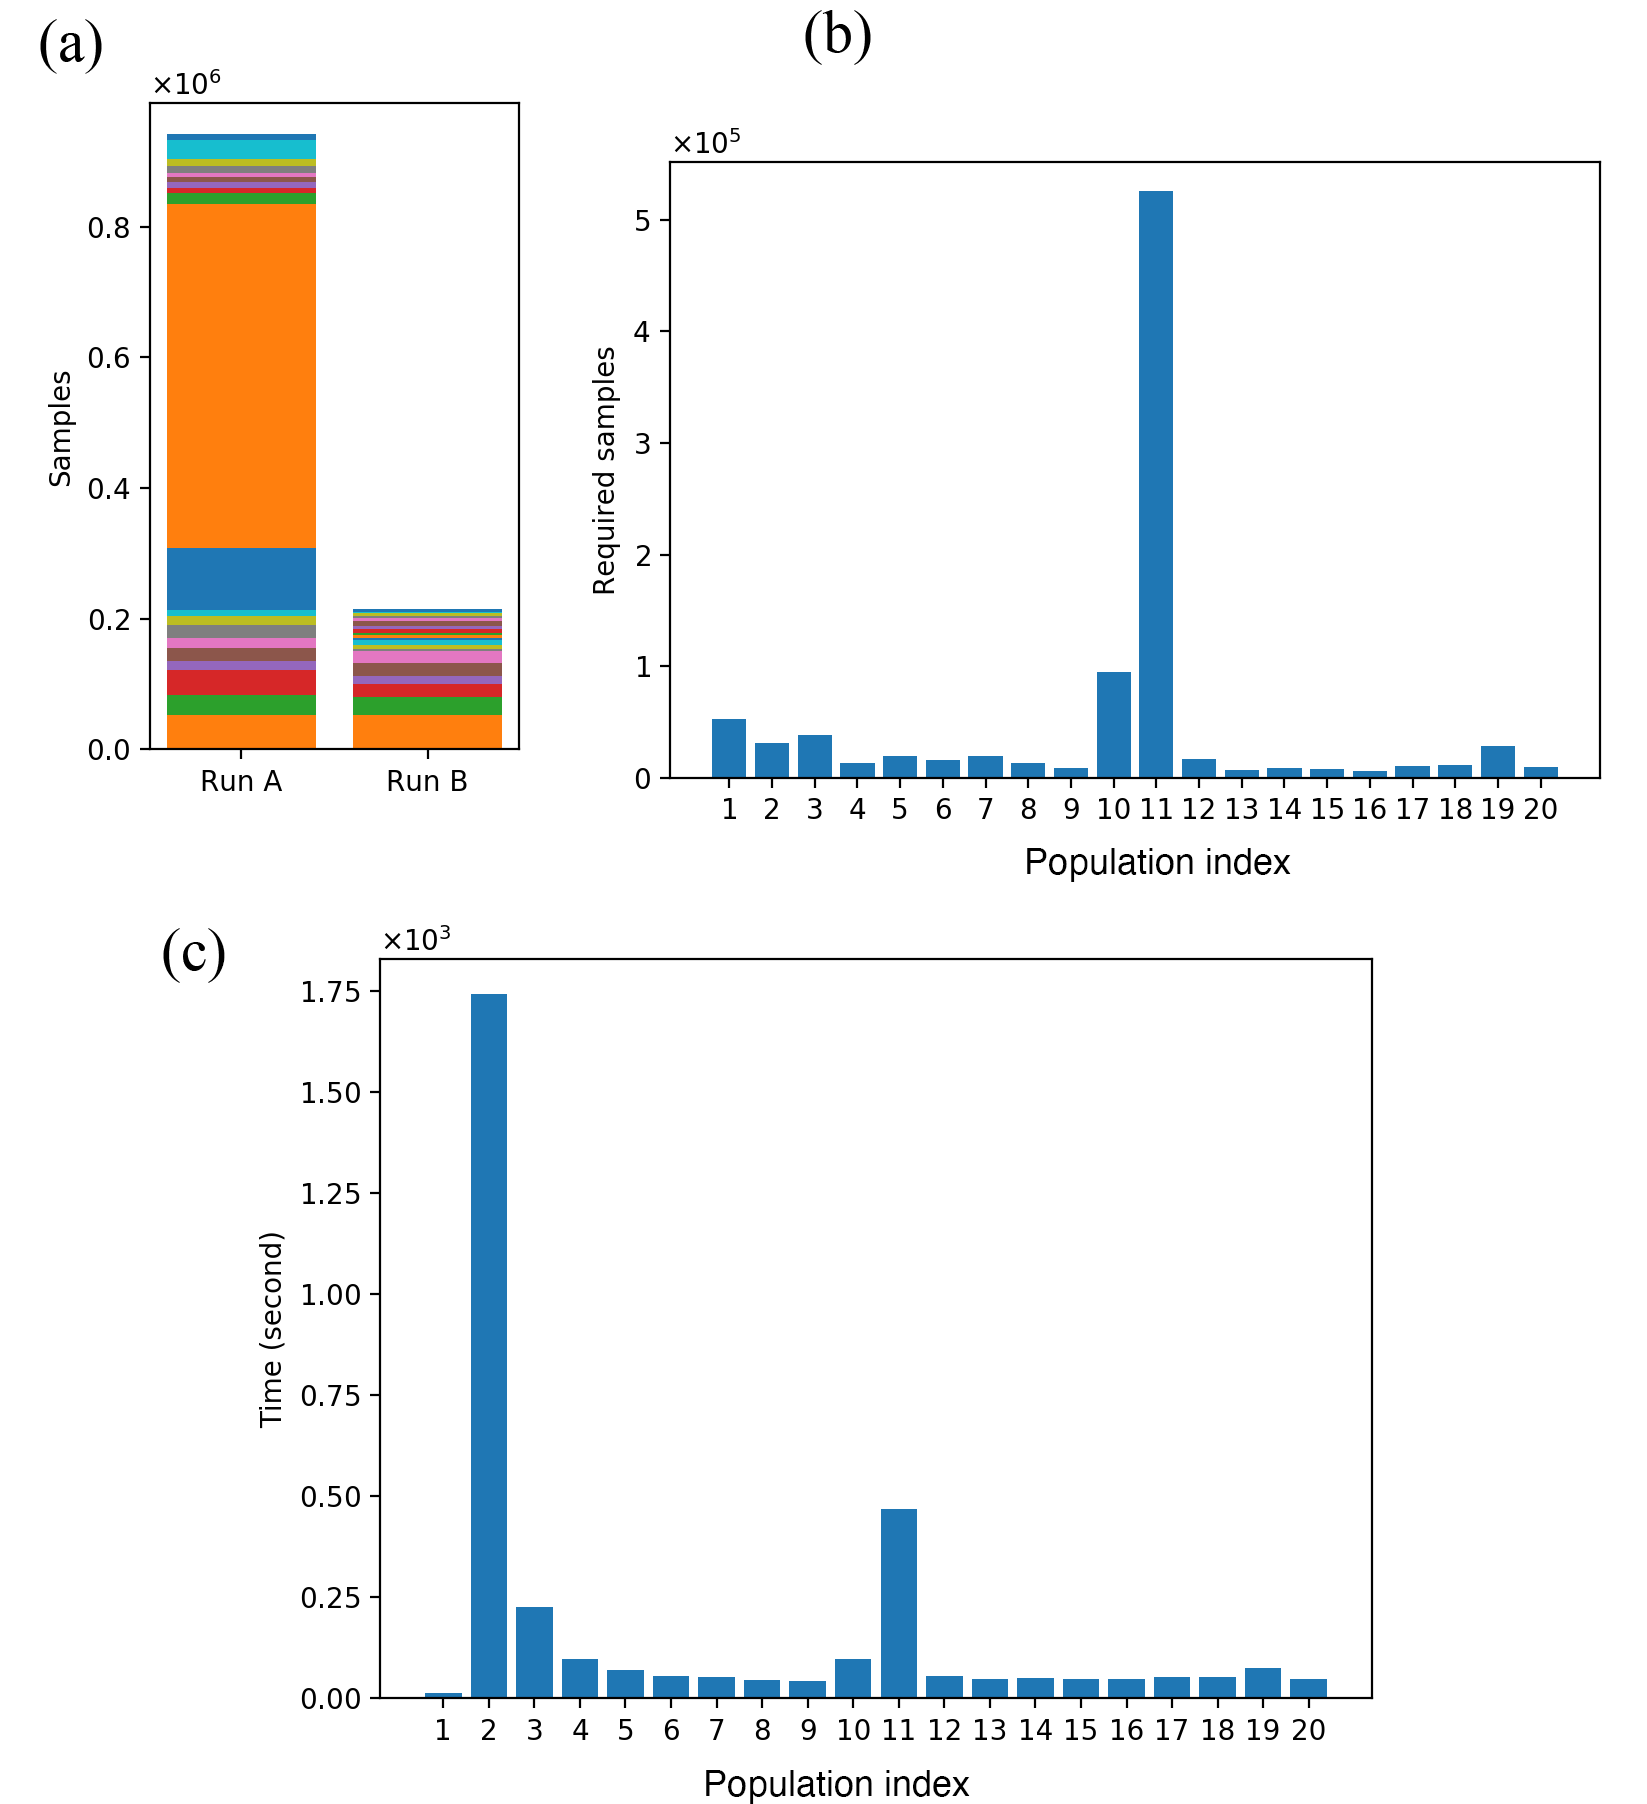
\includegraphics{fig/local_modes.png}}
    \end{center}

    \caption[Local optimum and abnormal pattern]{(a) Required sampling size for two example runs. Different colour represents different generation (from bottom to top: generation 1 to generation 20). Run A took huge amount of time in population 11. (b) Required sample in each generation of Run A. (c) Time-consumption in each generation of Run A}
    \label{fig:local_modes}
\end{figure}

To illustrate this, Two independent run, namely Run A and Run B, were chosen from the experiment of $p=24$ and visualised in Figure \ref{fig:local_modes} and Figure \ref{fig:local_para}. These two runs used identical options of the algorithm. Figure \ref{fig:local_modes} (a) shows the comparison of the required samples, where Run A converged to a local mode, and in population 11 took much more sample tires to move away from the local optimum (Figure \ref{fig:local_modes} (b)). Figure \ref{fig:local_para} compares the posterior density distribution before (t=9, cyan) and after (t=13, red) the jumping away: significant movement of concentrations in posterior density distributions are observed, especially in parameters from ODE 1, 2 and 4. An interning movement is that there are two concentrations in $\kappa_{\Phi\beta}$ and $\mu_\Phi$ when t=9, and the majority of particles are concentrated in the second concentration with high parameter values; when t=13, the second concentration distribution disappears and all particles are concentrated near zero.

\begin{figure}[h]
    \begin{center}
        \resizebox{1.0\hsize}{!}{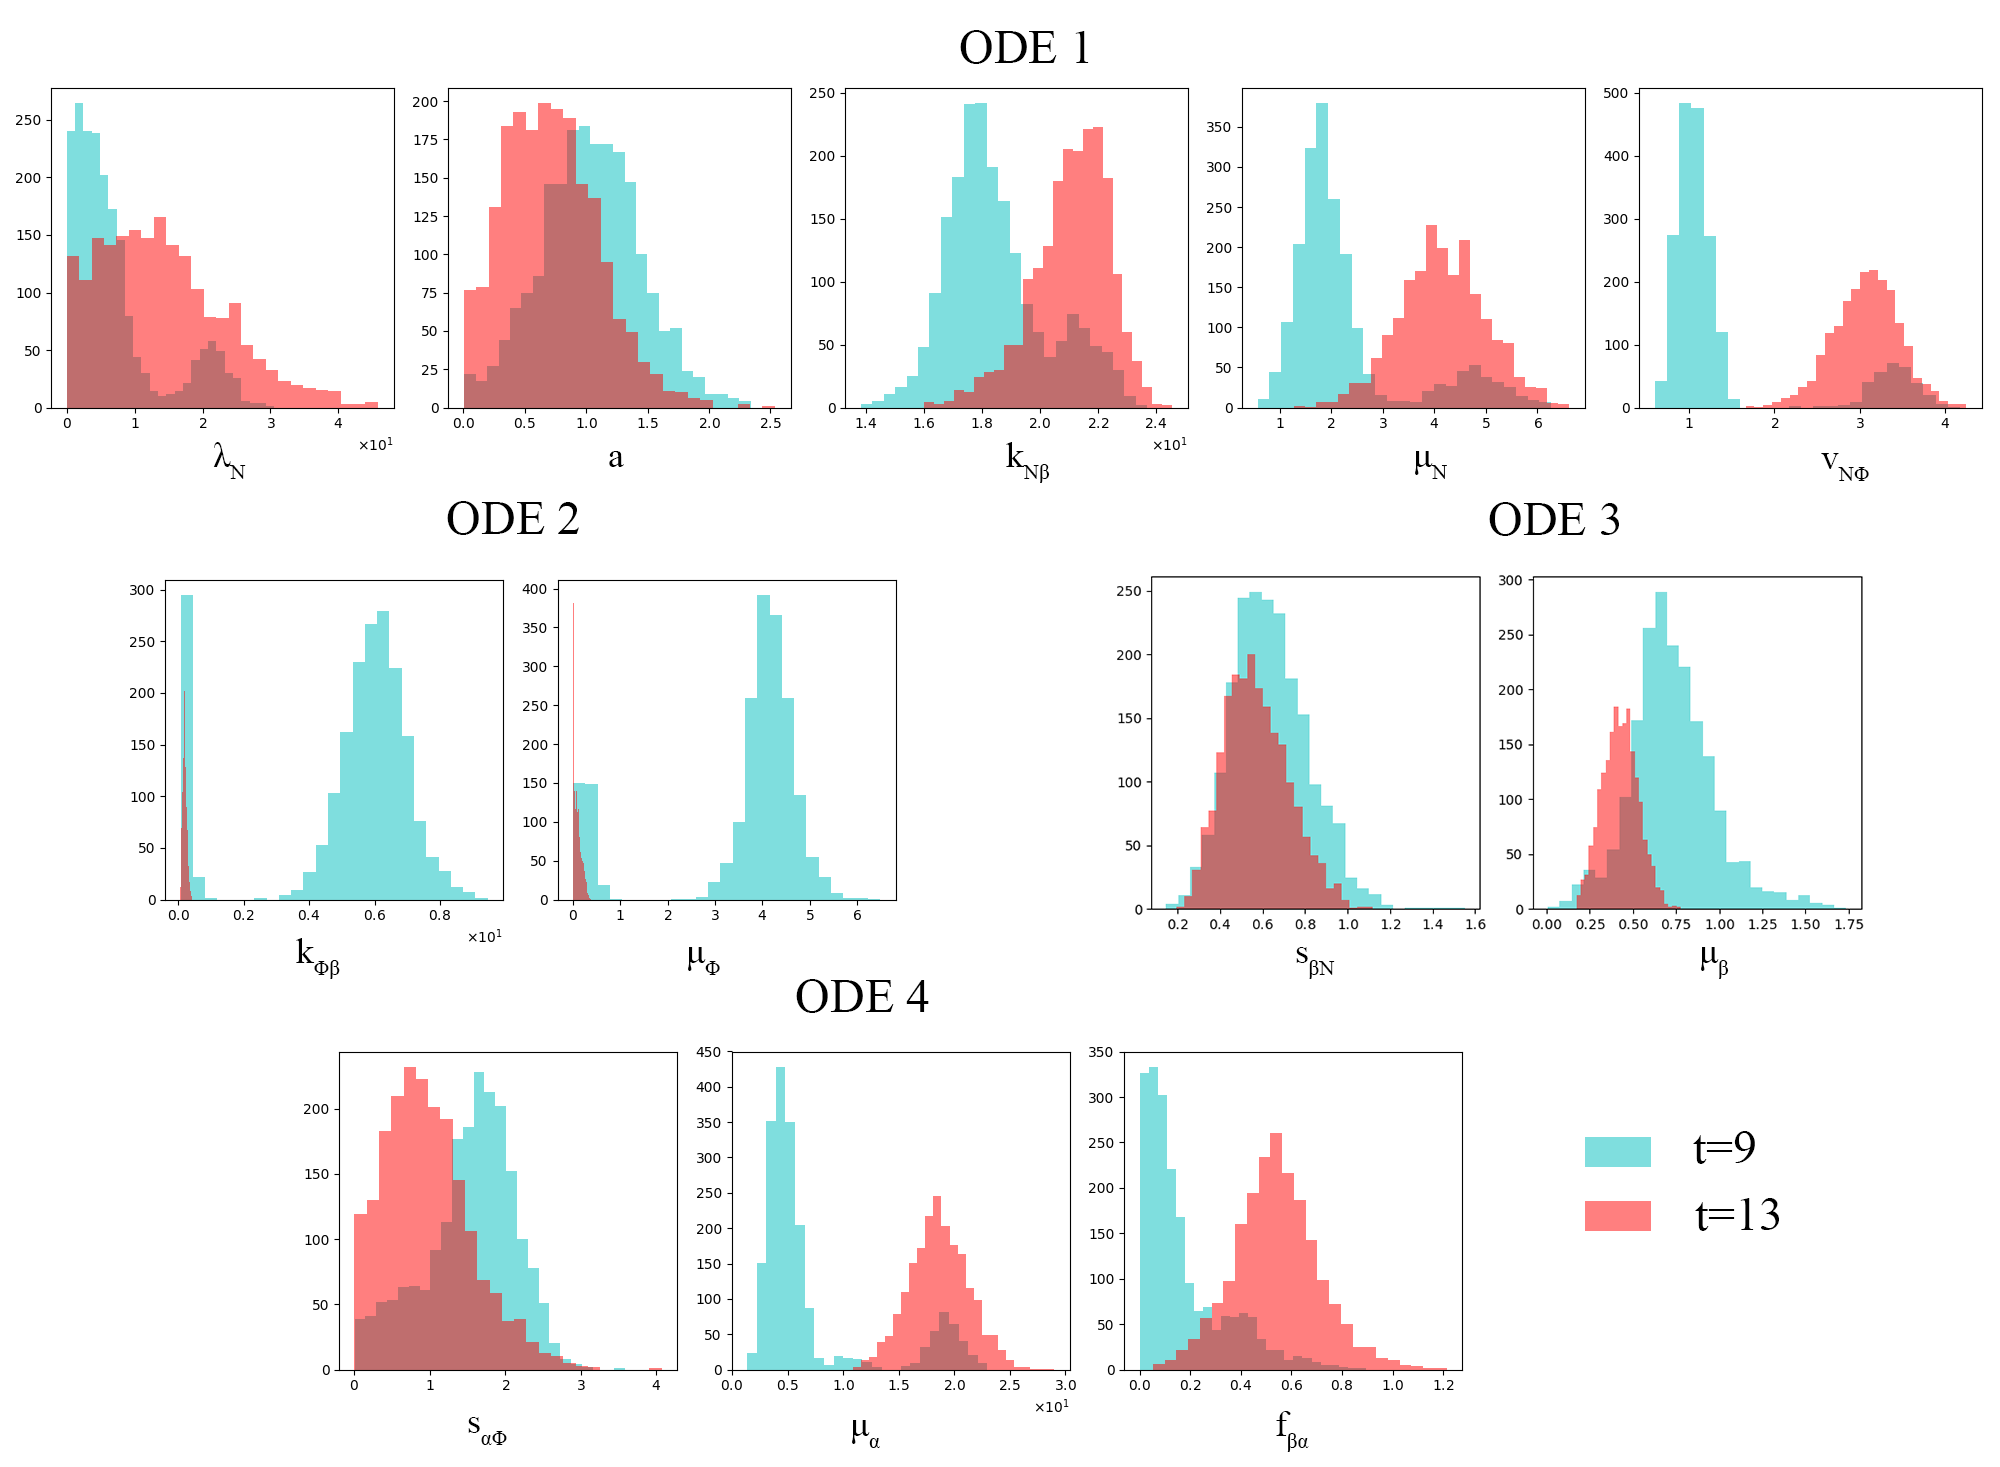
\includegraphics{fig/local_para.png}}
    \end{center}

    \caption[Parameter density distribution before and after the concentration movement in generation 11]{Parameter density distribution before (generation 9, cyan) and after (generation 13, red) the concentration movement in generation 11}
    \label{fig:local_para}
\end{figure}

Moreover, we found that the execution time was not ideally proportional to the sampling tires in that period of time, for both different repeated runs and different generations in a single run. From the same example, Figure \ref{fig:local_modes} (b) and (c) show the non-linear relationship between execution time and sample tries in different generations. Apart from 1st and 2nd generation, generation 3 to 20 show a general linear relationship i.e. $T_t\propto n_t$, where $t$ is the population index, $T_t$ is the execution time of generation $t$ and $n_t$ is the required samples in generation $t$. However, this relationship does not hold for the first two generations. Generation 1 is to draw samples from prior, but it is done with high efficiency as only a small amount of time are taken; generation 2 takes an unusually large amount of the, but it does not require much more samples. The abnormal execution time of generation 1 and two are observed in all other runs, where for $p=24$ generation 1 usually takes c. 16s and generation 2 takes c. 1600s. This is believed to be related to the initialisation of the algorithm. 

Additionally, by observing CPU frequency and load curve in-time while running the program, we found that the parallelised part is limited to the sampling, calculation and criterion test process. Some reduction calculations and preparation work for the next generation (e.g. calculation of the new epsilon values, normalisation of data, fit of multivariate kernel) are serial. The database I/O is also serial.

% A possible explain to these phenomenons can be that the median epsilon schedule results in different threshold strategies due to the randomness in the sampling process, thus results in different approximate convergency paths for different runs. Some runs that are stuck in a local optimum and require smaller target epsilon will take huge amount of samples to move away from the local optimum. This have been observed when the distribution of posterior is plotted before and after jumping away from local modes (FIGURE and more explain). Also, time spent in each sample using sanme number of cores is not constant in our case, which might be a result of the parallel schedule; ideally a serial run using only one core will see a nearly constant time spent in every particle.



% \section{Profiling}

% The performance could also be analysed given a profiling report. The second experiment profiles the program to reveal the detailed time consumption for each operation and the possible bottleneck, according to which we could find the hot-spot of program and given possible suggestions on improving the performance.

% In this case, profile tools \verb|cProfile| and \verb|yappi| is used in PyCharm IDE.

% \subsubsection{Results}

% [profiling results: hot-spot and possible improvements]
